\documentclass{beamer}
\usetheme{Pittsburgh}

\usepackage{amsmath}

\title{Problema da Mochila Binária}
\author{Fernando Gomes, Leonardo Holtz}
\institute{Universidade Federal do Rio Grande do Sul}
\date{}

\begin{document}

\begin{frame}

\titlepage

\begin{figure}
    \centering
    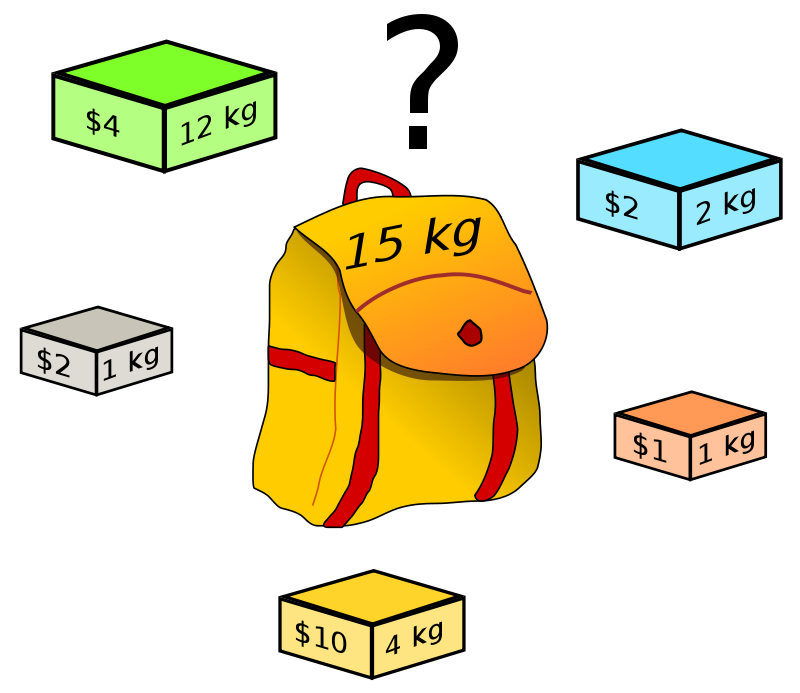
\includegraphics[scale=0.1]{Knapsack.png}
\end{figure}

\end{frame}

\begin{frame}
\frametitle{Sumário}
\tableofcontents
\end{frame}

% CARACTERIZAÇÃO DO PROBLEMA
\section{Caracterização do problema}

\begin{frame}
\frametitle{Definição intuitiva}

    Dado um conjunto de itens, com cada item tendo um peso
    e um custo, qual a escolha de itens tal que a soma de seus pesos é menor
    que a capacidade de uma mochila a soma de seus custos é a maior possível?

\end{frame}

\begin{frame}
\frametitle{Definição matemática}

    Dados uma mochila com capacidade máxima $W$, um conjunto de $n$ itens $x_{1}, x_{2}, ..., x_{n}$,
    cada um com um peso $w_{i}$ e um valor $v_{i}$:\\

    \begin{equation*}
        \text{maximizar} \sum_{i=1}^{n} v_{i} x_{i}
    \end{equation*}

    \begin{equation*}
        \mbox{sujeito a } \sum_{i=1}^{n} w_{i} x_{i} \leq W \mbox{ e } x_{i} \in \{0,1\}
    \end{equation*}

    Neste caso, $x_{i}$ representa o número de instâncias do item $i$ dentro da mochila.

\end{frame}

\begin{frame}
\frametitle{Aplicações}

Aplicações e blabalblabla

\end{frame}

%%%%%%%%%%%%%%%%%%%%%%%%%%%%%%%%%%%%%%%%%%%%%%%%%%%%%%

% PROVA QUE PERTENCE A NP
\section{Problema da mochila binária $\in$ NP}
\begin{frame}
\frametitle{Problema da mochila binária $\in$ NP}
\end{frame}

\subsection{Algoritmo de verificação}
\begin{frame}
\frametitle{Algoritmo de verificação}
\end{frame}

\subsection{Análise de complexidade}
\begin{frame}
\frametitle{Análise de complexidade}
\end{frame}


% PROVA QUE PERTENCE A NP-DIFICIL
\section{Problema da mochila binária $\in$ NP-difícil}
\begin{frame}
\frametitle{Problema da mochila binária $\in$ NP-difícil}
\end{frame}

\subsection{Problema NP-difícil usado}
\begin{frame}
\frametitle{}
\end{frame}

\subsection{Redução inst A para inst B}
\begin{frame}
\frametitle{Redução inst A para inst B}
\end{frame}

\subsection{Algoritmo de redução}
\begin{frame}
\frametitle{Algoritmo de redução}
\end{frame}

\subsection{Análise da complexidade}
\begin{frame}
\frametitle{Análise da complexidade}
\end{frame}

\section{Referências}
\begin{frame}
\frametitle{Referências}
\end{frame}

\end{document}

